\documentclass[tikz,border=5pt]{standalone}
\usepackage{xcolor}
\usepackage{tikz}
\usepackage{amsmath, amssymb}
\usepackage{lmodern}
\usepackage[T1]{fontenc}
\usepackage{pgfplots}

\begin{document}

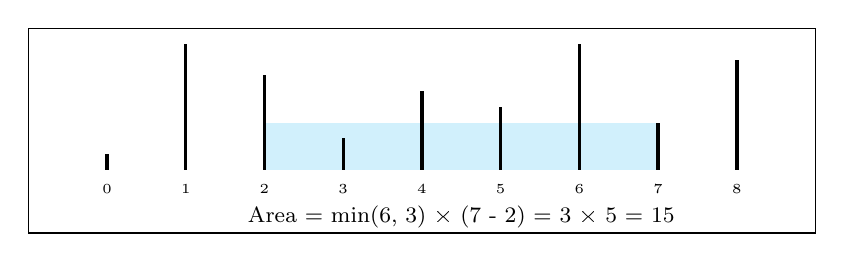
\begin{tikzpicture}[x=1cm, y=0.2cm]

  \draw[fill=white] (-1, -4) rectangle (9, 9);

  % Highlight water between index 2 and 7 (min height is 3)
  \fill[cyan!30, opacity=0.6] (2,0) rectangle (7,3);
  
  % Wall heights
  \foreach \x/\h in {0/1, 1/8, 2/6, 3/2, 4/5, 5/4, 6/8, 7/3, 8/7} {
    \draw[very thick] (\x,0) -- (\x,\h);  % thin vertical walls
    \node at (\x,-1.2) {\tiny \x};         % index labels
  }


  % Label with formula
  \node at (4.5,-3) {\footnotesize Area = min(6, 3) × (7 - 2) = 3 × 5 = 15};

\end{tikzpicture}


\end{document}
